\makeatletter
\def\input@path{{../}}
\makeatother
\documentclass[../master_thesis.tex]{subfiles}
\begin{document}
\chapter{Solvent Effect}\label{chap:Solvent_effect}
The goals of computational chemistry is to both approximate systems and to be
able to make predictions with regards to these approximations. In the previous
chapter \ref{chap:} I showed one of the ways to get good approximations of systems, now i
will talk about the set of systems that will be the focus for this thesis,
solvation models.
\section{Outlining the problem}
Solvation models describe one or more molecules (substrate) surrounded by
a set of other molecules (solvent). Most reactions of interest occur in a
solvent where the geometry, energy and kinetics of the reactants and products
are affected by their environment\cite{Mennucci:2018}.

We can describe the total Hamiltonian $\hat{H}_{sol}$ of a solvent-solute system as
\cite{Tomasi:1994wt}:
\begin{equation}\label{eq:Hsolvent}
  \hat{H}_{sol} = \hat{H}_0 + \hat{V}_{sol}
\end{equation}
where $H_0$ is the gas phase Hamiltonian (in vacuo) and $\hat{V}_{sol}$ is the
potential arising from the interactions between solvent and solute. These
interactions can be considered as perturbations to the in vacuo system.
The \ac{SE} of the system is as follows \cite{Tomasi:1994wt}
\begin{align}\label{eq:solSE}
  \hat{H}_{sol}\Psi^{(f)} = E^{(f)}\Psi^{(f)}
\end{align}
Where $f$ denotes the degree of  rigidity of the interactions (0 being with
completely static solvent molecules and rigidity decreasing with increasing
index). In most practical uses, we are interested in the polarization interaction
between the solvent and solute, meaning that one can replace the wave function $\Psi$ with the
total charge distribution of the solute $\rho_{\mathrm{tot}}$
\cite{Tomasi:1994wt}
\begin{align}
  \begin{split}\mathbb{}
      \rho_{\mathrm{tot}}(\rvec ; \vec{Q}) &=
      \rho_{\mathrm{nuc}}(\rvec, \vec{Q})
      + \rho_{\mathrm{el}}(\rvec ; \vec{Q}) \\
      \rho_{\mathrm{nuc}}(\rvec ; \vec{Q}) &=
      \sum_{\alpha} Z_{\alpha} \delta\left(\rvec
      - \vec{Q}_{\alpha}\right) \\
      \rho_{\mathrm{el}}\left(\vec{q}_{1} ; \vec{Q}\right) &=
      -\int\left|\Psi^{(f)}(\boldsymbol{q}, \vec{Q})\right|^{2}
      \mathrm{d}\vec{q}_{2} \ldots \mathrm{d}\boldsymbol{q}_{N_{\mathrm{el}}}
  \end{split}
\end{align}
Where $\alpha$ is an index that iterates over all the nuclei of the molecule,
$Z_{\alpha}$ is the nuclear charge of each nucleus, $\vec{q}_1, ..., \vec{q}_{N_{el}}$
represents the coordinates of the electrons, $\vec{Q}_{\alpha}$ represents the
coordinates of the nuclei and $\rvec$ is a vector variable describing a point
in three dimensions.

There are four main interactions affected by solvent effect which one might be
interested in solving. These are Electrostatic interactions, cavitation,
changes in dispersion and changes in bulk solvent structure \cite{Cramer:2004}.
In this thesis we work mostly with the electrostatics interactions of the
solute-solvent interface and the reaction field they create.

\subsection{The primitive Approach}
Our aim is to be able to simulate this system in an appropriate way, such that
the models let us predict rates, mechanisms and other specific processes which
occur in solutions \cite{Tomasi:1994wt}.
One can describe the solvation model in either an explicit or implicit way. In
this thesis I will focus on the implicit models, although I will give some
background in the explicit model.
A straightforward approach to the model is to try to, for example, make a
system of a \ce{Li^+} cation surrounded by water molecules. Here arises two
questions; how many water molecules should we add, and, in which positions
should we place them. Certainly one could say that we could just have enough
water molecules to surround the cation in one layer of them,  and just do a
geometry optimization \cite{Jensen:2017} on the system in order to get the
orientation and position of these water molecules.

Let us put the molecules in a cube-like fashion around the cation, with each
water molecule in a face of the cube, totaling 6 water molecules. In total we
would have 7 molecules, 19 nucleus and 62 electrons to optimize over. Using the
\ac{BO} approximation and \ac{DFT} we could solve the electronic part of the
problem in only three dimensions, but we would still need to work with
$57 (19\cdot3d)$ dimensions for the geometry of the nuclei. Even if we did do this
optimization and calculated the different interactions of this system, we would
find out that this approximation is very far from the truth.

If we look at the system we can see that this set of 7 molecules is suspended in
vacuum, which is not what we are trying to simulate. the water molecules at
the edge would not behave as if they were in solution, but as if they were in
gas phase. We are trying to simulate a \ce{Li^+} cation in a water solution.
We can add additional layers of water molecules to diminish the error. But
just adding a single layer of water molecules in a cube-like manner would
increase the amount of molecules to $31$ with a nuclear wave function of
$31\cdot3d$ dimensions. Adding more layers one after the other would end up
reducing the error to a neglectable level, as the amount of water molecules on
the surface will scale quadratic manner compared to the cubic scaling of the
water molecules inside the volume. This also means that the size of the system
would be too big to realistically work with in \ac{QM} and we would be forced to
calculate the effects as statistical averages over phase space
\cite{Cramer:2004}.


\subsection{Reaction Field}\label{Reaction_field}
Let us consider a system where a solute $A$ with a dipole moment $\vec{\mu}_A$ is
introduced to a solvent $S$ where each solvent molecule $S_i$ has its own dipole
moment $\vec{\mu}_{S_i}$. On equilibrium the different $S_i$  would be placed
randomly, giving an average electric field of zero. When $A$ is introduced, its
$\vec{\mu}_A$ will induce an electric field that will affect all the
$\vec{\mu}_{S_i}$ of the $S_i$. The $S_i$ will reorient themselves so that their
$\vec{\mu}_{S_i}$ lie along the electric field induced by $\vec{\mu}_A$. This is
so that they are in a more energetically favorable position in the electric
potential of the field induced by $\vec{\mu}_A$, but in doing this, they will
act against their own electric field and lose conformational freedom, which will
cost energy. This will, in turn, change the electric field of $S$ so that it no
longer behaves uniformly. The electric field of $S$ will then affect $A$ so that
$\vec{\mu_A}$ lies along the new electric field of $S$ for the same reason
stated above, using free energy in doing so \cite{Cramer:2004}.

The process outlined above will repeat itself until the energy gain from
reorienting $A$ and $S$ is outweighed by the required energy of such a
reorientation. The energy at such a point is equal to half the total interaction
energy between $S$ and $A$ \cite{Cramer:2004}. The new field obtained at the
equilibrium position of this interaction is called the Reaction field $U_r$ for
the interaction of $A$ and $S$.

\section{Explicit solvation models}

The explicit method is necessary when the solvent molecules' geometry and states
are important to the measurement of the interactions of the substrate
\cite{Cramer:2004}.
One way to simplify the problem is to partition the system into two parts, the
solvent, modeled using molecular mechanics (MM) and the solute, modeled using
\ac{QM}, this method is called MM/QM \cite{Mennucci:2018}.

The main point of this model is that the energy contribution from the solvent
can be described as a sum of bonding and non-bonding contributions
\cite{Cramer:2004} where the solvent bonds are described as springs
\cite{Mennucci:2018} and the atoms as weights. The bonding contributions can be
divided into bending, stretching and torsion of the bonds. Both the bending
and the stretching of the bonds can be described with the Harmonic Oscillator
(HO) and the torsion with a periodic function \cite{Mennucci:2018}. The
non-bonding interactions can be described with Coulombs law, or other equvalent
expressions of potentials, with the atoms as point charges. More information on
this can be read on \cite{Cramer:2004, Jensen:2017}.

\section{Implicit solvation models}
Most implicit models describe the solvent $S$ as a Linear isotropic continuum
characterized by the static dielectric constant $\epsinf$ characteristic
of the bulk of $S$ \cite{Tomasi:1994wt, FossoTande:2013ka}. In this continuum
only the electrostatic interactions are significant \cite{Tomasi:1994wt} meaning
that the interaction potential $\hat{V}_{int}$ in Equation \ref{eq:Hsolvent}
becomes an electrostatic potential $\hat{V}_{\sigma}$ \cite{Tomasi:1994wt}:

\begin{equation}
  \hat{V}_{\mathrm{int}}=\hat{V}_{\sigma}\left(\mathbf{q}, \mathbf{Q},
  \rho_{tot}, \epsinf\right)=\sum_{\alpha} Z_{\alpha} U_r
  \left(\mathbf{Q}_{\alpha}\right)-\sum_{i} U_r\left(\mathbf{q}_{i}\right)
\end{equation}
Where $U_r$ is the Reaction field potential.
The contribution of the interaction between $S$ and $A$ to the total energy
$E^{(f)}$ is given by
\begin{equation}
  W_{tot} = \int_{\real^3}\Psi^{(f)\star}\hat{V}_{\sigma}\Psi^{(f)}\text{d}q...\text{d}q_{N_{el}}
  = \braket{\rho_{tot}(\rvec)|U_r(\rvec)}
\end{equation}
This means that determining the reaction potential as well as knowing the coordinates
of the different particles will solve the Equation \ref{eq:solSE}.
These continuum models are also part of the \ac{PCM} classification of solvent
models.
Since we are looking at the effect the charge distribution of a solute has on
the interaction potential, we set up a Poisson equation. We also know that the change in
the potential must also be related to the dielectric constant that characterizes
the continuum $\epsilon$. We try to find the solution to the following
electrostatic potential equation
\begin{equation}
  \nabla\left( \epsilon(\rvec) \nabla U(\rvec)\right) = -4\pi\rho_{tot}
\end{equation}
Where $U(\rvec)$ is the electrostatic potential of the interaction between
the solute and the solvent. If $\epsilon$ is a constant we can move it outside
of the gradient operation and solve the Poisson equation with an effective $\rho$
\begin{equation}
  \nabla^2U(\rvec)=\frac{-4\pi}{\epsilon}\rho_{tot}
\end{equation}

\subsection{Cavity}\label{Cavitytitle}
All continuum models make use of a cavity in which the solute $A$ resides
\cite{Tomasi:1994wt, Cramer:2004, Tomasi:2005ipa}. The shape of the cavity
must be defined so it includes the whole molecule $A$ and its charge distribution.
Although, since the charge distribution of any molecule persists to infinity there
will always be an overlap with the charge distributions of the medium in real
systems. The charge that is not contained within the cavity is often called
escaped charge \cite{Tomasi:2005ipa}.

The size of the cavity is critical to the calculated results of the model, if
the cavity is too big the solvation effects are dampened, if it is too small
various errors may arise in the computation of the interactions to be studied
\cite{Tomasi:1994wt}. It is accepted that the cavity shape should closely
resemble the shape of the molecule itself \cite{Tomasi:2005ipa}. There are two
main ways of defining the shape and size of the cavity. These are (1) regular
shapes and (2) molecular shapes.

Regular shapes such as spheres, cylinders and ellipsoids have the advantage of
faster and simpler computations than molecular shapes. The fact that the cavity
should resemble the molecule and its charge distributions still stands, and it
is not realistic to assume that all molecules have regular shapes (apart from
maybe single atoms and linear molecules) \cite{Tomasi:2005ipa}

Molecular shapes give a better representation of the solute in the solvent due
to the fact that they more closely follow the shape of the solute molecule.
There are three main molecular shapes I wish to mention:
interlocking spheres, surfaces traced by solvent probes and isodensity surfaces.

\subsubsection{Molecular Surface shapes}

\paragraph{The Interlocking spheres model}
The interlocking spheres model is an extension of the regular shape model. In
this we create a set of spheres with radii $R_i$ that can be centered in the
nuclei of the molecule. Other centers can be in functional groups, so that they envelope a whole group,
or in specially designated spaces around the molecule so that the give an accurate
representation of the parts of the substrate molecule the solvent has access to
\cite{Tomasi:1994wt}. The latter is explained more in the next section.

The consensus for $R_i$ is that it has to be close to the \ac{vdW} radius
$R_{vdw}$ of the atom the sphere is centered in. One of the most used radii for
this  the $R_{vdw}$ used is the Bondi radii \cite{doi:10.1021/j100785a001,
Tomasi:2005ipa} multiplied by a coefficient $f$ that is close to 1. The
following relation holds
\cite{Tomasi:1994wt}
\begin{equation}
  R_i = fR_{vdw}
\end{equation}
where $f$ has been found to be, by statistical analysis, $f = 1.2 \pm 0.1$ in order to
yield the best results. Its value is $1.2$ for water while it can vary with
other solvents \cite{Tomasi:1994wt}. Although this only stands for neutral
solutes. Some results imply that the best radius for cations is the covalent
radius and the best one for anions is the ionic radius \cite{Tomasi:1994wt}.
\paragraph{Solvent probe tracing surfaces}\label{Spts}
This family of surfaces are based on the interlocking spheres model in that a
solvent probe (normally a spherical probe) is rolled around the Interlocking
sphere surface to trace a new surface. The inwards facing face of the probe traces a surface
which the solvent cannot access. This surface is called the Solvent Excluded
Surface (SES) \cite{Tomasi:2005ipa, Mennucci:2018}.  One can think of this as
smoothing so as to not get polarization in areas around the molecule which should
not be accessible for the solvent. Both SAS and SES are shown in the following
figure \ref{fig:SASSEShomemade}
\begin{figure}[ht]
  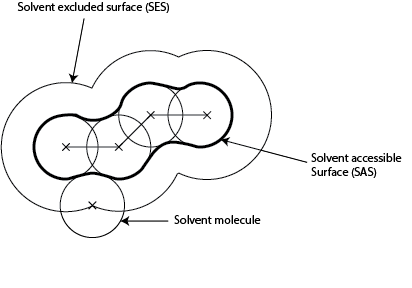
\includegraphics[width=\linewidth]{img/SASSES.png}
  \caption{SAS and SES surfaces}
  \label{fig:SASSEShomemade}
\end{figure}

\paragraph{Isodensity surfaces}
A third type of surface is one defined by a certain value of the charge density.
This is usually defined by setting a threshold value of the charge density for
which the surface will be drawn (usually $0.0004-0.001\ \text{a.u.}$)\cite{Tomasi:2005ipa}.


\subsection{Boundary conditions}
As stated before, in continuum models the solvent is represented by an isotropic
continuum defined by the dielectric constant $\epsinf$ characteristic to the bulk
solvent \cite{Tomasi:1994wt}. The interface between the solute and the continuum
is the cavity. One way to think of the value of the continuum is by defining a
function epsilon with the cavity as a boundary condition \cite{Tomasi:2005ipa, Tomasi:1994wt}:
\begin{equation}
  \epsilon(\rvec) =
  \begin{cases}
  \epsinf & \text{for} \ \rvec\in C\\
  1 & \text{for}\ \rvec \notin C
\end{cases}
\end{equation}
Where $C$ is the cavity. This definition brings forth a discontinuity on the
dielectric function. This makes solving the Poisson equation more difficult as
the gradient of the dielectric function is not defined at the surface of the
cavity. One way to bypass this problem is to partition the volume of the system
into two parts, one inside the cavity and one outside the cavity \cite{Tomasi:1994wt}.
Another assumption that is made is to say that we have an ideal cavity
\cite{Cramer:2004, Tomasi:1994wt}. In an ideal cavity, the electrostatic charge
is completelly contained within the cavity. This means that \cite{Tomasi:1994wt}
\begin{equation}
  \rho_{\mathrm{tot}}(\rvec)=0 \quad \rvec \notin C
\end{equation}
This lets us define the Poisson equation inside and outside the cavity as follows
\cite{Sorland, Tomasi:1994wt}:
\begin{align}
  \begin{split}
    \nabla^2U(\rvec) &= -4\pi\rho_{tot}(\rvec)\ \rvec\in C\\
    \epsinf\nabla^2U(\rvec) &= 0 \ \rvec \notin C
  \end{split}
\end{align}
Where, for a point $\vec{s}$ and a normal outwards vector $\vec{n}$ on the
surface of the cavity, the following conditions are true
\cite{Sorland, Tomasi:1994wt}:
\begin{align}
  \begin{split}
    U_{in}(\vec{s}) = U_{out}(\vec{s})\\
    \frac{\partial U_{in}}{\partial\vec{n}} = \epsinf\frac{\partial U_{out}}{\partial\vec{n}}
  \end{split}
\end{align}
Where $U(\rvec)$ is the sum of the potential of the substrate in vacuo
$U_{vac}$ and the reaction field potential $U_r$\cite{Sorland, FossoTande:2013ka}
\begin{equation}\label{eq:Utot}
  U(\rvec) = U_{vac}(\rvec) + U_r(\rvec)
\end{equation}

\subsection{Approaches to a solution}\label{approchessolv}
\subsubsection{ \ac{ASC}}
In this family of solutions we look at the classical electrostatics description
of the problem. we do this by defining an apparent charge distribution
$\sigma$ confined to the surface of the cavity $\Gamma$ \cite{Tomasi:1994wt, Tomasi:2005ipa}.
The apparent surface charge distribution at the boundary between two regions $i, j$
is defined as
\begin{equation}
  \sigma_{ij} = -(\vec{P}_j - \vec{P}_i)\cdot\vec{n}_{ij}
\end{equation}
where $\vec{n}_{ij}$ is the unit vector pointing from $i$ to $j$ and $\vec{P}$ is
the polarization vector of a region of constant isotropic permitivity (such as
the continuum in \ac{PCM}) defined as
\begin{equation}
  \vec{P}_i (\rvec) = - \frac{\epsilon_i - 1}{4\pi}\nabla U(\rvec)
\end{equation}
where $\epsilon_i$ is the permitivity constant of region $i$ \cite{Tomasi:2005ipa}.
In a solvation model we only have two regions, one inside and one outside. We
know that $\epso = 1$ so $\vec{P}_0 = 0$ leaving only the outside region to
construct $\sigma$. This gives us \cite{Tomasi:2005ipa}
\begin{equation}
  \sigma(\vec{s}) =\frac{\epsinf - 1}{4\pi\epsinf} \frac{\partial}{\partial\vec{n}} (U_{vac} + U_{\sigma})_{in}\ ;\ s \in \Gamma
\end{equation}
and we find the reaction potential of the apparent surface charge $U_{\sigma}$
with the following integral
 \begin{equation}
   U_{\sigma}(\rvec) = \int_{\Gamma}\frac{\sigma(\vec{s})}{\abs{\rvec - \vec{s}}} \text{d}\vec{s}\ ;\ s \in \Gamma
 \end{equation}
Which, if we divide the surface into a set of finite elements (tesserae
\cite{Tomasi:2005ipa, Sorland}) with set areas $A$ that are small enough to be able
to assume that $\sigma$ does not change inside each of these tesserae, will let us define the integral
as a sum over all the tesserae
\begin{equation}
   U_{\sigma}(\rvec) \simeq \sum_k\frac{\sigma(\vec{s}_k) A_k}{\abs{\rvec - \vec{s}_k}} \text{d}\vec{s}
   = \sum_k\frac{\sigma(q_k}{\abs{\rvec - \vec{s}_k}}
\end{equation}
Where $q_k$ is the point charge of each tesserae from the product of $sigma{\vec{s}_k}A_k$
\cite{Tomasi:2005ipa}.
Many slightly different types of \ac{ASC} have been implemented as of now. Some of these
are \ac{COSMO}, \ac{IEF} and \ac{SVPE}.

\paragraph{\ac{COSMO}}
In this version of \ac{ASC} we proceed as normal except that we define $\epsinf = \infty$.
This way we determine the {ac{ASC}} ($\sigma^{\star}$) by the local value of the electrostatic
potential instead of computing the normal component of its gradient \cite{Tomasi:2005ipa}.
We then scale $\sigma^{\star}$ as follows
\begin{equation}
  \sigma(\vec{s}) = \frac{\epsinf -1}{\epsinf + k}\sigma^{\star}(\vec{s})
\end{equation}
where $k$ is small \cite{Tomasi:2005ipa}.

\paragraph{\ac{IEF}}
In this method we define the electrostatic potentials in terms of Green integral
functions. The Green function $G(\vec{x}, \vec{y})$ is the potential produced at
a point $\vec{x}$ by a unit charge at $\vec{y}$ \cite{Tomasi:2005ipa}. We define
the electrostatic potentials as follows

\begin{equation}
\begin{aligned} U(x) &=\int_{R^{3}} G^{s}(x, y) \rho_{\mathrm{M}}(y) \mathrm{d} y \\
  U_{vac}(x) &=\int_{R^{3}} G(x, y) \rho_{\mathrm{M}}(y) \mathrm{d} y \\
  U_{r}(x) &=\int_{R^{3}} G^{R}(x, y) \rho_{\mathrm{M}}(y) \mathrm{d} y \end{aligned}
\end{equation}
where $G(\vec{x}, \vec{y})=1 /|x-y|$ is the green kernel for the operator
$-\nabla^2$, $G^s(\vec{x}, \vec{y})$  is the green function of
$-\nabla(\epsilon{\rvec}\nabla)$ and $G^{r}(x, y)=G^{\mathrm{s}}(\vec{x},
\vec{y})-G(\vec{x}, \vec{y})$. Then the reaction potential $U_r$ can be represented
as  \cite{Tomasi:2005ipa}

\begin{equation}
U_{\mathrm{R}}(x)=\int_{\Gamma} \frac{\sigma(\vec{y})}{|\vec{x}-\vec{y}|}
\mathrm{d} \vec{y} \forall \vec{x} \in R^{3}
\end{equation}
where the surface charge $\sigma$ is given by solving the following equation

\begin{equation}
\left[2 \pi\left(\frac{\epsilon+1}{\epsilon-1}\right)-D_{\mathrm{i}}\right] S_{\mathrm{i}} \sigma=-\left(2 \pi-D_{\mathrm{i}}\right) V_{vac}
\end{equation}
Where $S_{\mathrm{i}}$ and  $D_{\mathrm{i}}$ are two of the four components of the Calderon projector \cite{Tomasi:2005ipa}.

\paragraph{\ac{SVPE}}
The main focus of this method is that the solute charge distribution has a trailing
"tail" that reaches outside the surface \cite{Tomasi:2005ipa}. We define the
Reaction potential as consisting of a \ac{ASC} term $U_{\sigma}$ and a exterior
term $U_{\beta}$
\begin{align}
  \begin{split}
    U_r(\vec{x}) = U_{\sigma}(\vec{x}) + U_{\beta}(\vec{x})\\
    U_{\beta}(\vec{x}) = -\frac{\epsinf - 1}{\epsinf}\int_{ext} \frac{\rho_{tot}(\vec{y})}{\abs{\vec{x} - \vec{y}}} \text{d}\vec{y}
  \end{split}
\end{align}
Where $x, y$ are defined as above.

\subsubsection{Multipole expansion (MPE)}
In this solution we write the total electrostatic potential $U(\rvec)$ in terms
of Legendre polynomials. This way the potential is reduced to a set of two
spherical harmonics functions, one outside and one inside the cavity.
\begin{align}
  \begin{split}
    U_{in}(\rvec) &= \sum_{l=0}^{\infty}\frac{1}{r^{l+1}}\sum^l_{m=-l}B_{lm}Y^m_l(\theta, \phi) \\
    &+ \sum_{l=0}^{\infty}\frac{(l+1)(\epsinf - 1)}{l + (l+1)\epsinf} \frac{r^{l+1}}{a^{2l+1}}\sum^l_{m=-l}B_{lm}Y^m_l(\theta, \phi)\\
    U_{out}(\rvec) &=\sum_{l=0}^{\infty}\frac{2l+1}{l+(l+1)\epsinf}\frac{1}{r^{l+1}}\sum^l_{m=-l}B_{lm}Y^m_l(\theta, \phi)
  \end{split}
\end{align}
Where $Y^m_l$ is the spherical harmonics with angular momentum $l$ and projection
along the z-axis $m$, $a$ is the radius of the cavity and $B_{lm}$ is a set of
constants which need to be found \cite{Tomasi:1994wt}.


\subsubsection{Solving in \ac{MW}}\label{solmw}
Following Fosso-Tande \cite{FossoTande:2013ka} the cavity is defined as a atom
based interlocking spheres cavity (ABC-cavity). We start by defining a normal
signed distance function $s_i$ of a point $\rvec$ away from the surface of the
sphere $C_i$ with radius $R_i = 1.2\cdot R^{vdw}_i$ and centered on atom $i$ with
coordinate $\rvec_i$ \cite{FossoTande:2013ka}:
\begin{equation}
  s_i(\rvec) = \abs{r -r_i} - R_i
\end{equation}
The Cavity for the $i$-th atom is defined as
\begin{equation}
  C_i(\rvec) = 1 - \Theta(s_i(\rvec)) =\Theta(-s_i(\rvec))
\end{equation}
Where $\Theta$ is a heavyside-like function that enables to smoothly transition
from the inside of the cavity (value $1$), to the surface of the cavity (value
$\frac{1}{2}$) and to the outside of the cavity (value $0$)
\cite{Sorland, FossoTande:2013ka}. We use the error function $\erf(x)$ to define
$\Theta$ and a parameter $\sigma$ characterizing the width of the transition
between the inside and outside of the cavity.
\begin{equation}
  \Theta\left(s_i\right) = \frac{1}{2}\left(1 + \erf\left(\frac{s_i}
  {\sigma}\right)\right)
\end{equation}
The function for the complete set of interlocking spheres $C$ for a molecule
with $N$ atoms is given by
\begin{equation}
  C(\rvec) = 1 - \prod_{i=1}^N(1 - C_i(\rvec))
\end{equation}
This function can then be used further in creating a dielectric function
$\epsilon$ that switches smoothly from $\epso$ (permitivity of free space
with value $1$ \cite{FossoTande:2013ka}) to $\epsinf$ either with a linear
representation
\begin{equation}\label{eq:dielfuncexp}
  \epsilon(\rvec) = \epsinf  + (\epso - \epsinf)C(\rvec)
\end{equation}
or with an exponential representation
\begin{equation}\label{eq:dielfunclin}
  \epsilon(\rvec) =\epso\exp\left( \left(\log\frac{\epsinf}{\epso} \right)
  (1 - C(\rvec)) \right)
\end{equation}
Which gives itself better for computation of its $\log$-derivative
\cite{FossoTande:2013ka}
\begin{equation}\label{eq:logderepsexp}
  \nabla\log\epsilon(\rvec) = \frac{\nabla\epsilon(\rvec)}{\epsilon(\rvec)}
   = \left(\log\frac{\epso}{\epsinf} \right)\nabla C(\rvec)
\end{equation}
The log derivative of the linear dielectric function is expressed as
\begin{equation}\label{eq:logderepslin}
  \nabla \log(\epsilon (\rvec)) = \frac{\nabla\epsilon(\rvec)}{\epsilon(\rvec)}
  = \frac{(\epso - \epsinf)}{\epsilon(\rvec)}\nabla C(\rvec)
\end{equation}

With either of those dielectric functions, the \ac{GPE} can be constructed
\cite{Sorland, FossoTande:2013ka}
\begin{align}\label{eq:gpemw}
  \nabla\cdot (\epsilon(\rvec)\nabla U(\rvec)) &= -4\pi \rho_{tot}(\rvec) \\
  \nabla^2U(\rvec) &= -4\pi \frac{\rho_{tot}}{\epsilon(\rvec)} - \frac{\nabla
  \epsilon(\rvec)\cdot \nabla U(\rvec)}{\epsilon(\rvec)}
\end{align}
We define the effective charge distribution $\rho_{eff}$ and the surface charge
distribution $\gamma_s$ \cite{FossoTande:2013ka}
\begin{align}\label{eq:effrhogamma}
  \rho_{eff}(\rvec) &= \frac{1}{\epsilon(\rvec)}\rho_{tot}(\rvec) \\
  \gamma_s(\rvec) &= \frac{1}{4\pi}\frac{\nabla\epsilon(\rvec)}{\epsilon(\rvec)}\cdot\nabla U(\rvec)
\end{align}
and substitute them into Equation \ref{eq:gpemw}
\begin{equation}\label{eq:gpepractical}
  \nabla^2U(\rvec) = -4\pi\left( \rho_{eff}(\rvec) + \gamma_s(\rvec)\right)
\end{equation}
We get the total iteration potential $U(\rvec)$ between the substrate and the solvent by
applying the Poisson operator $\hat{\mathscr{P}}$ as defined in Equation
\ref{eq:Poissonopmw} to equation \ref{eq:gpepractical}
\begin{equation}
  U(\rvec) = \hat{\mathscr{P}}\left( \rho_{eff}(\rvec) + \gamma_s(\rvec)\right)
\end{equation}
We can then find the reaction potential following the Equation \ref{eq:Utot} and
rearranging it so we get the following.
\begin{equation}
  U_r(\rvec) = U(\rvec) - U_{vac}(\rvec)
\end{equation}
The reaction field energy is given as \cite{FossoTande:2013ka}
\begin{align}
  E_{tot} &= - E_{vac} + \frac{1}{2}E_r \\
  E_r = \braket{U_r | \rho_{tot}}\\
  E_{vac} = \braket{U_{vac}| \rho_{tot}}
\end{align}
Since the solution of the total potential has the potential in both sides of the
equation we will need to iterate with an initial guess. This will be explained
more thoroughly in Chapter \ref{chap:implementation}.

\section{Variational implementation}
Following Lipparini \cite{Lipparini:2010bg, Lipparini:2013} I'll arrive at a functional where
minimizing with respect to $U$ of the solvent energy contribution to
the total energy $G_s$ will give a way to determine $U_r$ variationaly.

Starting from the \ac{GPE} defined from \cite{FossoTande:2013ka} we project it
into a suitable space with test functions $\psi$

\begin{align}
  \begin{split}\label{eq:projectedgpe}
    &\nabla (\epsilon\nabla U) = -4\pi\rho\\
    &-\braket{\psi|\nabla |\epsilon\nabla U} = 4\pi \braket{\psi|\rho}
  \end{split}
\end{align}
Applying the following vector identity
\begin{equation}
\nabla (\psi \epsilon\nabla U)=\nabla \psi \epsilon \nabla U +  \psi \nabla \epsilon \nabla U +  \psi \epsilon\nabla^{2} U
\end{equation}
we get the integral
\begin{equation}
  -\int_{\real^3}\psi \nabla \epsilon \nabla U\text{d}r - \int_{\real^3}  \psi\epsilon \nabla^{2} U\text{d}r = \int_{\real^3} \nabla \psi \epsilon \nabla U\text{d}r - \int_{\real^3} \nabla (\psi \epsilon\nabla U\text{d}r)
\end{equation}
The test functions vanish on the surface of the cavity. Applying the Gauss' theorem \cite{Lipparini:2013} we can turn the rightmost integral into
an integral on the surface, thus vanishing. This gives us:
\begin{equation}
  -\braket{\psi|\nabla|\epsilon\nabla U} = \braket{\nabla \psi |\epsilon | \nabla U}
\end{equation}
which we substitute into Equation \ref{eq:projectedgpe}
\begin{equation}
  \braket{\nabla \psi |\epsilon | \nabla U} =  4\pi \braket{\psi|\rho}
\end{equation}
which lets us write the functional for the energy as \cite{Lipparini:2010bg}
\begin{equation}
  G(U) = \frac{1}{8\pi}  \braket{\nabla U |\epsilon | \nabla U} - \braket{U|\rho}
\end{equation}
We now find the gradient of the functional in order to minimize with respect to $U$
\begin{equation}
  \frac{\partial}{\partial U}G(U) = \frac{\partial}{\partial U}\frac{1}{8\pi}\braket{\nabla U|\epsilon|\nabla U} - \frac{\partial}{\partial U}\braket{U|\rho}
\end{equation}
Where if we set $\frac{\partial}{\partial U}G(U) = 0$ we get the \ac{GPE} from \cite{FossoTande:2013ka}
and thus we can use any type of minimization method to reach the right potential.

\begin{acronym}
\acro{AUS}[\href{https://www.sigma2.no/content/advanced-user-support}{AUS}]{Numerical Methods in Quantum Chemistry}
\acro{BO}{Born-Oppenheimer}
\acro{CTCC}[\href{http://www.ctcc.no}{CTCC}]{Centre for Theoretical and Computational Chemistry}
\acro{DC}{Dielectric Continuum}
\acro{DFT}{Density Functional Theory}
\acro{EFP}{Effective Fragment Potential}
\acro{EU}{European Union}
\acro{HF}{Hartree-Fock}
\acro{Hylleraas}[\href{https://www.mn.uio.no/hylleraas/english/}{Hylleraas}]{Hylleraas
  Centre for Quantum Molecular Sciences}
\acro{HPC}{High Performance Computing}
\acro{KTH}{Royal Institute of Technology}
\acro{LDA}{Local Density Approximation}
\acro{MCD}{Magnetic Circular Dichroism}
\acro{MCSCF}{Multiconfiguration Self Consistent Field}
\acro{MM}{Molecular Mechanics}
\acro{MW}{Multiwavelet}
\acro{NFR}{Norwegian Research Council}
\acro{NMQC}[\href{http://www.ctcc.no/events/conferences/2015/numeric-conference/}{NMQC}]{Numerical Methods in Quantum Chemistry}
\acro{NOTUR}[\href{https://www.notur.no/}{NOTUR}]{Norwegian Metacenter for Computational Science}
\acro{PCM}{Polarizable Continuum Model}
\acro{PI}{Primcipal Investigator}
\acro{QC}{Quantum Chemistry}
\acro{QM}{Quantum Mechanics}
\acro{QM/MM}{Quantum Mechanics/Molecular Mechanics}
\acro{ROA}{Raman Optical Activity}
\acro{SC}{semiconductor}
\acro{SCF}{Self Consistent Field}
\acro{SHG}{Second Harmonic Genertation}
\acro{STSM}{Short-term scientific mission}
\acro{TPA}{Two-Photon Absorption}
\acro{WP}{Work Package}
\acro{CBS}{Complete Basis Set}
\acro{TCG}{Theoretical Chemistry Group}
\acro{vdW}{van der Waals}
\acro{SE}{Schrödinger Equation}
\acro{PES}{Potential Energy Surface}
\acro{LCAO}{Linear Combination of Atomic Orbitals}
\acro{MRA}{Multi-Resolution Analysis}
\acro{NS}{Nonstandard}
\end{acronym}

\biblio
\end{document}
